\title{\textbf{Negative thermal expansion: nature and application}}
\author{Mnatsakanov Anton}
\date{National Technical University of Ukraine “Igor Sikorsky Kyiv Polytechnic Institute”
Kiev, Ukraine}

\documentclass[10pt, a4paper, twocolumn]{article}
\usepackage[left=1.6cm,right=1.8cm,top=2.0cm,bottom=2.8cm,bindingoffset=0cm]{geometry}
\usepackage[russian,ukrainian,english]{babel}
\usepackage{scrextend}
\usepackage[T1,T2A]{fontenc}
\usepackage[utf8]{inputenc}
	\usepackage[english,ukrainian,russian]{babel}
	\usepackage{amsmath,amssymb}
	\usepackage{array,tabularx}
	\usepackage{graphicx}
    \graphicspath{{C:/Users/anmnm/Desktop/4-cours/DIPLOM/obzor/images/}}
	\usepackage{moreverb}
	\usepackage{xcolor}
	\usepackage{color}
	\usepackage{hyperref}
	\hypersetup{%
		colorlinks=true,
		linkbordercolor= red,
		urlbordercolor=green,
    }%for hyperrefs
%------------------ 
\usepackage[many]{tcolorbox}
	\newtcbox{\mylib}{enhanced,nobeforeafter,tcbox raise base,boxrule=0.4pt,top=0mm,bottom=0mm,
	  right=0mm,left=4mm,arc=1pt,boxsep=2pt,before upper={\vphantom{dlg}},
	  colframe=green!50!black,coltext=green!25!black,colback=green!10!white,
	  overlay={\begin{tcbclipinterior}\fill[green!75!blue!50!white] (frame.south west)
	    rectangle node[text=white,font=\sffamily\bfseries\tiny,rotate=90] {TYP} ([xshift=4mm]frame.north west);\end{tcbclipinterior}}}

%------------------  
\newcolumntype{Y}{>{\centering\arraybackslash}X}
%------------------  
\usepackage{lstautogobble}  % Fix relative indenting
%\usepackage{color}          % Code coloring
\usepackage{zi4}            % Nice font
	\definecolor{bluekeywords}{rgb}{0.13, 0.13, 1}
	\definecolor{greencomments}{rgb}{0, 0.5, 0}
	\definecolor{redstrings}{rgb}{0.9, 0, 0}
	\definecolor{graynumbers}{rgb}{0.5, 0.5, 0.5}

	\usepackage{listings}
	\lstset{
  basicstyle=\ttfamily,
  columns=fullflexible,
  frame=single,
  breaklines=true,
  postbreak=\mbox{\textcolor{red}{$\hookrightarrow$}\space},
  }
%------------------
\usepackage[object=vectorian]{pgfornament} %%  http://altermundus.com/pages/tkz/ornament/index.html
		\usepackage{tikz}
		\newcommand{\sectionlinetwo}[2]{%
		\nointerlineskip \vspace{.5\baselineskip}\hspace{\fill}
		{\color{#1}
		\resizebox{0.5\linewidth}{2ex}
		{{{\begin{tikzpicture}
		\node  (C) at (0,0) {};\node (D) at (9,0) {};
		\path (C) to [ornament=#2] (D);
		\end{tikzpicture}}}}}%
		\hspace{\fill}
		\par\nointerlineskip \vspace{.5\baselineskip}}

  %\newcommand{\img}[4]{\center{\includegraphics[width=#1\linewidth]{#2}}\captionof{figure}{#3}\label{#4}}
\newcommand{\img}[4]{\includegraphics[width=#1\linewidth]{#2}\caption{#3}\label{#4}}


%-----------------------------
\usepackage{tcolorbox}
\tcbuselibrary{skins,breakable}
\usetikzlibrary{shadings,shadows}%preambule
%-----------------------------
\newtcbox{\mybox}[1][red]{on line,
arc=0pt,outer arc=0pt,colback=#1!10!white,colframe=#1!50!black,
boxsep=0pt,left=1pt,right=1pt,top=2pt,bottom=2pt,
boxrule=0pt,bottomrule=1pt,toprule=1pt}

\newtcbox{\xmybox}[1][red]{on line,
arc=7pt,colback=#1!10!white,colframe=#1!50!black,
before upper={\rule[-3pt]{0pt}{10pt}},boxrule=1pt,
boxsep=0pt,left=6pt,right=6pt,top=2pt,bottom=2pt}
%-----------------------------
\usepackage{tikz}
\usetikzlibrary{shapes.callouts}
%-----------------------------
\definecolor{amber}{rgb}{1.0, 0.75, 0.0}
\definecolor{babyblue}{rgb}{0.54, 0.81, 0.94}
%-----------------------------

	\usepackage[framemethod=TikZ]{mdframed}
	\usetikzlibrary{calc}
	\makeatletter
	\newlength{\mylength}
	\xdef\CircleFactor{1.1}
	\setlength\mylength{\dimexpr\f@size pt}
	\newsavebox{\myboxx}
	\newcommand*\circled[2][draw=blue]{\savebox\myboxx{\vbox{\vphantom{WL1/}#1}}\setlength\mylength{\dimexpr\CircleFactor\dimexpr\ht\myboxx+\dp\myboxx\relax\relax}\tikzset{mystyle/.style={circle,#1,minimum height={\mylength}}}
	\tikz[baseline=(char.base)]
	\node[mystyle] (char) {#2};}
	\makeatother
%-----------------------------
\usepackage{verbatim}

\usetikzlibrary{arrows,shapes,backgrounds}
%-----------------------------
\usepackage{multicol}
%-----------------------------
%\usepackage[most]{tcolorbox}
	\definecolor{orang}{RGB}{255,155,0}
	\newtcolorbox[auto counter,number within=section]{caja}[1][]{
	enhanced jigsaw,colback=white,colframe=orang,coltitle=orang,
	fonttitle=\bfseries\sffamily,
	sharp corners,
	detach title,
	leftrule=10mm,
	% What you need %%%%%%%%%%%%
	underlay unbroken and first={\node[below,text=black,anchor=east]
	at ([xshift=-5.5pt]interior.base west) {\Huge  \textbf{!}};},
	%%%%%%%%%%%%%%%%%%%%%%%%
	breakable,pad at break=1mm,
	#1,
	code={\ifdefempty{\tcbtitletext}{}{\tcbset{before upper={\tcbtitle\par\medskip}}}},}
%-----------------------------
\newcommand{\enum}[2]{\begin{tikzpicture}
\node (0,0) {\begin{minipage}[m]{0.95\textwidth}
#1
\end{minipage} };
\node [opacity=0.05] (0,0) {\scalebox{10.0}{\textcolor{red}{\emph{#2}}}};
\end{tikzpicture}}
%-----------------------------
%-----------------------------
%-----------------------------
%-----------------------------
%-----------------------------
%-----------------------------
%-----------------------------
%-----------------------------
%-----------------------------
%-----------------------------
\graphicspath{{C:/Users/anmnm/Desktop/4-cours/DIPLOM/obzor/images/}}
\usepackage{xurl}
\usepackage[super,comma,sort&compress]{natbib}
\usepackage{abstract}
\renewcommand{\abstractnamefont}{\normalfont\bfseries}
\renewcommand{\abstracttextfont}{\normalfont\small\itshape}
\usepackage{lipsum}

%%%%%%%%%%%%%%
% References %
%%%%%%%%%%%%%%

 \usepackage{blindtext}
\usepackage{hyperref}
\hypersetup{colorlinks=true, urlcolor=blue, linkcolor=blue, citecolor=blue}

\begin{document}

%%%%%%%%%%%%%%%%%%%%%%%%%%%%%%%%%%%%%%%%%%%%
  
%\section{Name}
    
   
%%%%%%%%%%%%%%%%%%%%%%%%%%%%%%%%%%%%%%%%%%%%
\twocolumn[\maketitle
    \begin{abstract}
      Negative thermal expansion (NTE) is an uncommon physical and chemical phenomenon in which some materials shrink when heated rather than expand like most other materials.  За последнее несколько лет было достигнуто значительное развитие в области материалов NTE. Это открыло новую область композитов пр  создании которых  используют материалы NTE в качестве компенсаторов теплового расширения. \\ 

      Keywords -- thermal expansion, negative thermal expansion,  invar and  covar materials,...
    \end{abstract}]
%%%%%%%%%%%%%%%%%%%%%%%%%%%%%%%%%%%%%%%%%%%% 
 \clearpage
\section{Introduction}

Some materials, when the temperature rises, do not demonstrate expansion, but, on the contrary, contraction, that is, they have a negative coefficient of thermal expansion $ \alpha $ (which at lower temperatures is typical for any polar crystal). For some substances, this manifests itself in a rather narrow temperature range, such as, for example, as the best known material with NTE is water at 0 ... 4 $^{\circ} $ С this property is also present in other substances and materials, for example fluoride scandium ($ ScF_3 $), zirconium tungstate ($ZrW_2O_8$), some CFRPs, the range is very wide. This behavior is also demonstrated by ordinary rubber. At ultra-low temperatures, quartz, silicon and a number of other materials behave in a similar way.
%%%%%%%%%%%%%%%%%%%%%%%%%%%%%%%%%%%%%%%%%%%%

%\section{Invar and Covar effects}

%...\\
%There are also invar alloys (ferro-nickel), which have a coefficient of thermal expansion close to zero in a certain temperature %range.
%...\\

%The effect of the disappearance of thermal expansion of a material occurs due to the fact that magnetostriction precisely compensates for thermal expansion. \\

%Thermal expansion is one of the fundamental properties of all solids.
%But quite often, some materials exhibit properties of shrinkage when heated and under constant pressure. These are materials with negative thermal expansion (NTE). NTE materials are of great practical importance, since they allow
%regulate the thermal expansion of the material to
%some specific meaning, usually achieved through the formation of composites.

%...

\section{Thermal expansion in different crystals}


%%%%%%%%%%%%%%%%%%%%%%%%%%%%%%%%%%%%%%%%%%%%
\section{Applications}
Some materials which undergo NTE have a range of potential engineering, photonic, electronic, and structural applications. For example, if one were to mix a negative thermal expansion material with  material which expands on heating (typical, normal materials), it is possible to use it as a thermal expansion compensator what might allow for forming composites with tailored or even close to zero thermal expansion. \\ 

Combining a material with positive heat expansion and a material with negative heat expansion can allow to regulate the thermal expansion of composites or even to obtain compositions with warm expansion close to zero, ie with increasing body temperature will not change its size. The change in the object will not occur because the negative and positive thermal expansion will compensate for the other to some extent when the temperature changes. Adjusting the total coefficient of thermal expansion (CTE) to certain values  can be achieved by changing the volume fractions of different materials involved in the thermal expansion of the composition.\\ 

\begin{figure}[h!]
\center{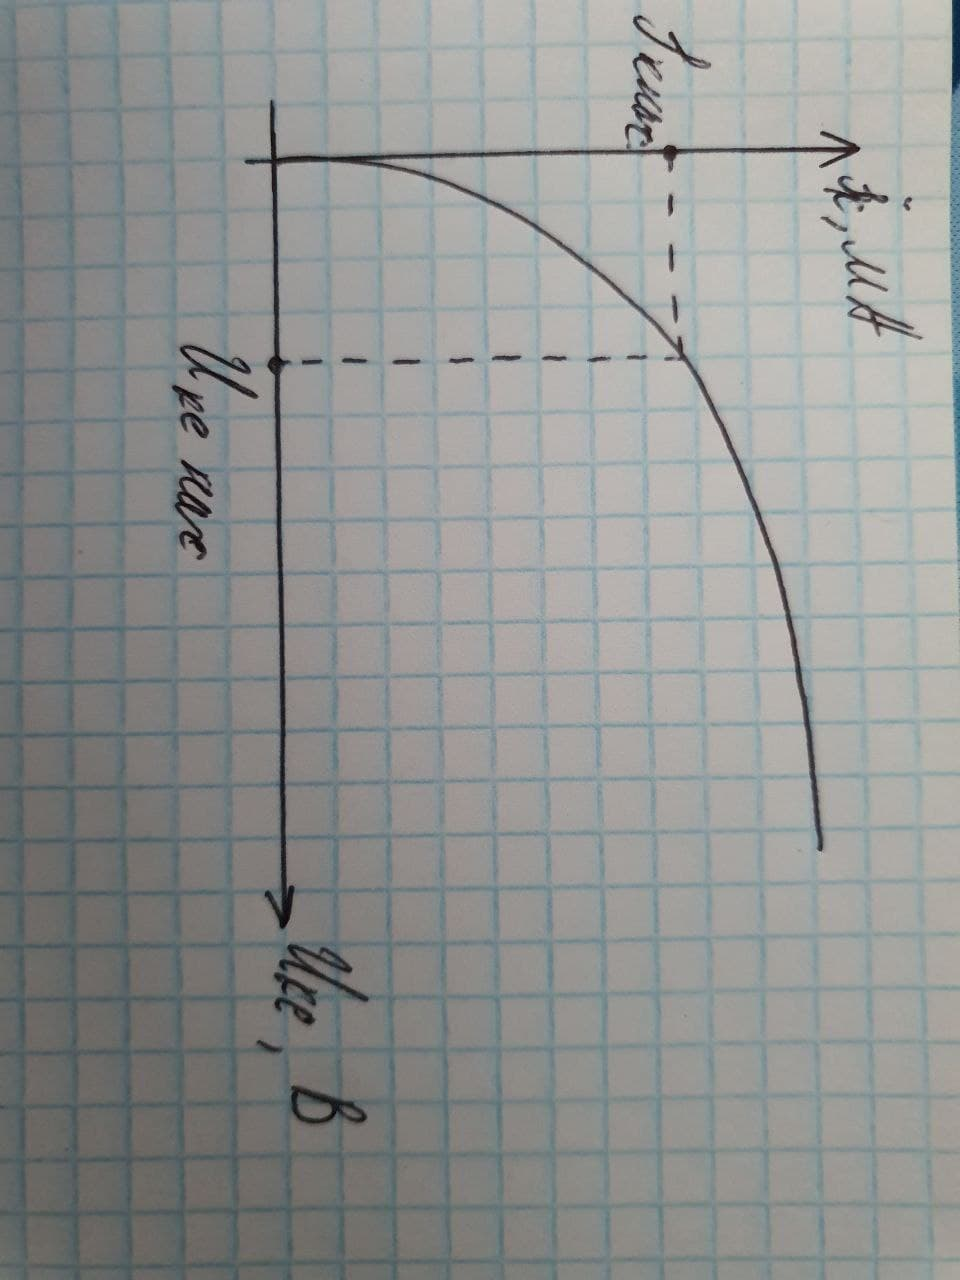
\includegraphics[width=0.5\linewidth]{2.jpg}}
\caption{Schematic of anisotropic thermal expansion in the silicates. As the shaded layers undergo thermal expansion, they are pulled closer together in the direction perpendicular to the layers, which causes significant thermal contraction in this direction.}
\label{ris2}
\end{figure}

A practically important group of negative- or low-expansion materials is formed by different materials (silicates) of various kinds such as $LiAlSiO_4$ ($\beta$-eucryptite)\cite{lit6}, $Li_2Al_2Si_nO_{4+2n}$ ($\beta$-spodumenes) \cite{lit4} and $Mg_2Al_4Si_5O_{18}$ (cordierite)\cite{lit2}. Such silicates are sometimes distinguished from other NTE materials having flexible bonds\cite{lit5}. Here, they are grouped together, emphasizing their common features that non-expansive covalent bonds and thermally excited lattice deformation consuming open spaces play an essential role in NTE. These material contain two-dimensional sheets composed of ionic bonds such as Li–O and Mg–O; the sheets are connected by strong covalent bonds such as Al–O and Si–O. Because the ionic bonds lengthen with increasing temperature, expansion occurs in two dimensions within the sheets. Due to the rigidity of the covalent bonds, the sheets are forcibly pulled closer together, as shown schematically in Fig.\ref{ris1}. Consequently, significant NTE appears in one direction to the perpendicular to thermal-expansive sheets (Fig.\ref{ris2}). Although volume thermal expansion can be either positive or negative in this mechanism, many materials show net negative (although not large) volume thermal expansion. Large anisotropy in the thermal expansion restricts the practical use of these materials. For example, their performance as thermal-expansion compensators depends strongly on their morphology\cite{lit1}.
\begin{figure}[h!]
\center{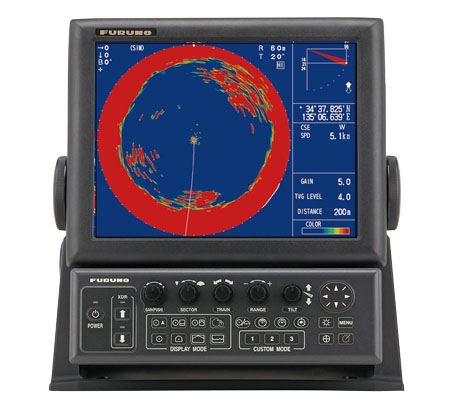
\includegraphics[width=0.6\linewidth]{1.jpg}}
\caption{Axial and aggregate thermal expansion of $\beta$-eucryptite \cite{lit6}.}
\label{ris1}
\end{figure}

Materials with near-zero CTE, i.e. constant characteristics over a large temperature range, are most widely used in precision instruments, since any change in one or another parameter leads to errors and undesirable deviations. But also in everyday life, materials with a CTE close to zero are required. Vitrified ceramic cooktops, such as Ceran cooktops, have to withstand high temperature gradients and rapid temperature changes during cooking, as only certain parts of the cooking surface get hot, while other parts remain close to ambient temperature. Generally, due to their brittleness, temperature gradients in glass can lead to cracks. However, the glass ceramic used in hobs consists of several different layers, some of which have positive and others negative thermal expansion. The expansion of the different phases compensates each other and the volume of the ceramic does not change much with temperature and cracking is avoided.Materials with near-zero CTE, i.e. constant characteristics over a large temperature range, are most widely used in precision instruments, since any change in one or another parameter leads to errors and undesirable deviations. But also in everyday life, materials with a CTE close to zero are required. Vitrified ceramic cooktops, such as Ceran cooktops, have to withstand high temperature gradients and rapid temperature changes during cooking, as only certain parts of the cooking surface get hot, while other parts remain close to ambient temperature. Generally, due to their brittleness, temperature gradients in glass can lead to cracks. However, the glass ceramic used in hobs consists of several different layers, some of which have positive and others negative thermal expansion. The expansion of the different phases compensates each other and the volume of the ceramic does not change much with temperature and cracking is avoided.\\ 

In everyday life, an example of the need for materials with controlled thermal expansion is dental fillings. If the fillings have a tendency to expand by an amount different from the expansion of the teeth, e.g. when drinking hot or cold, this can cause toothache, which can be very uncomfortable. However, if dental restorations are made of composite material containing a mixture of materials with positive and negative thermal expansion, the overall expansion can be exactly matched to the expansion of the tooth enamel.

%%%%%%%%%%%%%%%%%%%%%%%%%%%%%%%%%%%%%%%%%%%%















%%%%%%%%%%%%%%%%%%%%%%%%%%%%%%%%%%%%%%%%%%%% References 
\begin{thebibliography}{9}
\bibitem{lit1} \href{https://scholar.google.com/scholar_lookup?journal=Mater.+Sci.+Eng.&author=C+N+Chu&author=N+Saka&author=N+P+Suh&volume=95&publication_year=1987&pages=303&issn=00255416&doi=10.1016/0025-5416(87)90523-4&}{Chu C N, Saka N. and Suh N P. Mater. Sci. Eng. 1987;95:303. doi: 10.1016/0025-5416(87)90523-4.}  
 
 \bibitem{lit2} \href{https://scholar.google.com/scholar_lookup?journal=J.+Am.+Ceram.+Soc.&author=M+E+Milberg&author=H+D+Blair&volume=60&publication_year=1977&pages=372&issn=0002-7820&issn=1551-2916&doi=10.1111/jace.1977.60.issue-7-8&}{Milberg M E. and Blair H D. J. Am. Ceram. Soc. 1977;60:372. doi: 10.1111/jace.1977.60.issue-7-8.}

 \bibitem{lit3} Yu. M. Poplavko. Polar bonds self-ordering and negative thermal expansion.  
Kiev, Ukraine, 2021.

 \bibitem{lit4} \href{https://scholar.google.com/scholar_lookup?journal=J.+Am.+Ceram.+Soc.&author=W+Ostertag&author=G+R+Fischer&author=J+P+Williams&volume=51&publication_year=1968&pages=651&issn=00027820&issn=15512916&doi=10.1111/jace.1968.51.issue-11&}{Ostertag W, Fischer G R. and Williams J P. J. Am. Ceram. Soc. 1968;51:651. doi: 10.1111/jace.1968.51.issue-11.}

 \bibitem{lit5} \href{https://scholar.google.com/scholar_lookup?journal=Inorg.+Chem.&author=A+W+Sleight&volume=37&publication_year=1998&pages=2854&issn=0020-1669&issn=1520-510X&doi=10.1021/ic980253h&}{Sleight A W. Inorg. Chem. 1998;37:2854. doi: 10.1021/ic980253h.}
 
 \bibitem{lit6} \href{https://scholar.google.com/scholar_lookup?journal=J.+Am.+Ceram.+Soc.&author=F+H+Gillery&author=E+A+Bush&volume=42&publication_year=1959&pages=175&issn=0002-7820&issn=1551-2916&doi=10.1111/jace.1959.42.issue-4&}{Gillery F H. and Bush E A. J. Am. Ceram. Soc. 1959;42:175. doi: 10.1111/jace.1959.42.issue-4.}

 \bibitem{lit7} \href{https://iopscience.iop.org/article/10.1088/0034-4885/79/6/066503}{Dove, Martin T; Fang, Hong (2016-06-01). "Negative thermal expansion and associated anomalous physical properties: review of the lattice dynamics theoretical foundation". }

 \bibitem{lit8} 

 \bibitem{lit9} 

 \bibitem{lit10} 

 \bibitem{lit11} 

\end{thebibliography}

\end{document}


      

  